\documentclass[aspectratio=169]{beamer}
\mode<presentation>
%\usetheme{Warsaw}
%\usetheme{Goettingen}
\usetheme{Hannover}
%\useoutertheme{default}

%\useoutertheme{infolines}
\useoutertheme{sidebar}
\usecolortheme{dolphin}


\setbeamersize{sidebar width left=0pt} % to remove the sidebar
\beamertemplatenavigationsymbolsempty % To remove the navigation symbols on the bottom right.
\setbeamersize{text margin left=10mm,text margin right=10mm} % Specify margins

\usepackage{amsmath}
\usepackage{amssymb}
\usepackage{listings}
\usepackage{enumerate}
\usepackage{hyperref}
\hypersetup{
    colorlinks=true,
    linkcolor=blue,
    filecolor=magenta,      
    urlcolor=cyan,
}

%%%%For drawing graphs
% a nice font
\usepackage{kpfonts}

% basic text stuff
\usepackage[utf8]{inputenc}
\usepackage[T1]{fontenc}

\usepackage{tikz} % main tikz package
\usepackage{tikz-network} % for network / graph utilities

% for a nicer colorscheme
%\input{colors.tex} % By nemo.fournier https://nemo.kiwi/latex.html#h3_colors
%%%%%%%%%%%%%%%%%%%%%%%%%%%%%%%

\begin{document}
 
\urlstyle{same}

%some bold math symbosl
\newcommand{\Cov}{\mathrm{Cov}}
\newcommand{\Var}{\mathrm{Var}}
\newcommand{\brho}{\boldsymbol{\rho}}
\newcommand{\bSigma}{\boldsymbol{\Sigma}}
\newcommand{\btheta}{\boldsymbol{\theta}}
\newcommand{\bbeta}{\boldsymbol{\beta}}
\newcommand{\bmu}{\boldsymbol{\mu}}
\newcommand{\bW}{\mathbf{W}}
\newcommand{\one}{\mathbf{1}}
\newcommand{\bH}{\mathbf{H}}
\newcommand{\by}{\mathbf{y}}
\newcommand{\bolde}{\mathbf{e}}
\newcommand{\bx}{\mathbf{x}}

\newcommand{\cpp}[1]{\texttt{#1}}

%--------------------------------------------------
\providecommand{\abs}[1]{\lvert#1\rvert}
\providecommand{\norm}[1]{\lVert#1\rVert}
\providecommand{\Blue}[1]{\textcolor{blue}{#1}}
\providecommand{\Red}[1]{\textcolor{red}{#1}}  
\providecommand{\Purple}[1]{\textcolor{purple}{#1}} %for notations
\newcommand{\celsius}{\ensuremath{^\circ}C}
\newcommand\thfore{\mathord{\therefore}\,}
%------------------------------------------------------------------

\title{Lecture 6. Hamilton Paths and Circuits~\footnote{
  This terminology comes from a game, called the Icosian puzzle, invented in 1857 by the
Irish mathematician Sir William Rowan Hamilton.}
}
%\author{
\includegraphics[width=.8\textwidth,height=.7\textheight]{lecture1-fig0.jpg}}

\date{ }
%------------------------------------------------------------------

\frame[plain]{\titlepage}

\begin{frame}[plain]{} 


\begin{center}
  {\bf Does a path or circuit exist that uses every vertex exactly once?
  }
\end{center}

\vspace{.1in}

\begin{columns}[t] % contents are top vertically aligned
\begin{column}[c]{5cm}

  \begin{center}
     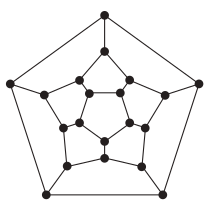
\includegraphics[height=4cm]{./img/lecture6-fig1a.png}
  \end{center}
   
  \end{column} \pause
  \begin{column}[c]{5cm}
      \begin{center}
        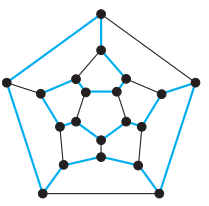
\includegraphics[height=4cm]{./img/lecture6-fig1b.png}
      \end{center}
  \end{column}
  \end{columns}
\vspace{.2in}


\begin{itemize}
           \item A \Blue{Hamilton path} in a graph $G$ is a \Red{simple path} {\bf containing 
              every vertex of $G$ exactly once}. 
               That is, a Hamilton path is a path that
              visits every vertex exactly once 
              (allowing for revisiting edges).
           \item A \Blue{Hamilton circuit} in a graph $G$ 
           is a Hamilton path that starts and ends on the same vertex.
          \end{itemize}
    
\end{frame}


\begin{frame}[plain]{}

{\bf Example 6.1.} Which graphs have a Hamilton circuit or, 
if not, a Hamilton path?%Rosen, sec 10.5, p734-735, Ex 5

\begin{center}
        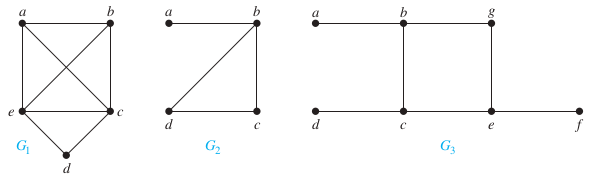
\includegraphics[height=3.7cm]{./img/lecture6-fig2.png}
 \end{center}
 \pause 
 
 {\bf Solution:} 
 $G_1$ has a Hamilton circuit: $a, b, c, d, e, a.$ 
 There is no Hamilton circuit in $G_2$ (this can
   be seen by noting that any circuit containing every vertex must contain 
   the edge $\{a, b\}$ twice),
   but $G_2$ does have a Hamilton path, namely, $a, b, c, d$. 
   $G_3$ has neither a Hamilton circuit nor a
    Hamilton path, because any path containing all vertices 
    must contain one of the edges $\{a, b\}$, $\{e, f\}$, and $\{c, d\}$ more than once.

\end{frame}

\begin{frame}[plain]{}

 {\bf Question:} Is there a simple way to determine 
  whether a graph has a Hamilton circuit or path? \pause
  Ansewr is "No".
  \medskip
  
  \begin{quote}
    Finding efficient algorithm = ultimate computer science glory.
  \end{quote}
  
  The best algorithms known so far for finding a Hamilton circuit
   in a graph, or determining that no such circuit exists, have 
   \Red{exponential worst-case time complexity} (in the number of vertices of the graph), 
   which is incredibly slow for sufficiently large graphs.
    \medskip
    
  Finding an algorithm that solves this problem with polynomial worst-case time
complexity would be a major accomplishment,
 and you would probably be given every single computer science award in existence.
 
\end{frame}

\begin{frame}[plain]{}

Some Properties:
\begin{itemize}
  \item A graph with \Red{a vertex of degree one} cannot have a Hamilton circuit, 
   because in a Hamilton circuit, each vertex is incident with two edges in the circuit.\pause
  \item  If a vertex in the graph has \Red{degree two}, then
      \Red{both edges} that are incident with this vertex must be part of 
      any Hamilton circuit. \pause
  \item When a Hamilton circuit is being constructed and this circuit has passed through 
  a vertex, then \Red{all remaining edges} incident with this vertex, other than the two used 
  in the circuit, can be \Red{removed} from consideration. \pause
 % \item A Hamilton circuit \Red{cannot contain a smaller circuit} within it. \pause
\end{itemize}

{\bf Example 6.2.} 
Use the above properties to explain why the following graphs don't have Hamilton circuits.
%Rosen, sec 10.5, p735, Ex 6

  \begin{center}
        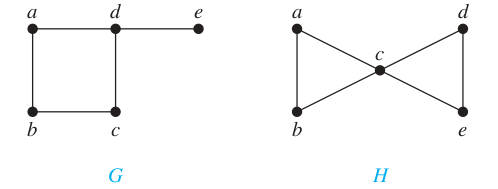
\includegraphics[height=3cm]{./img/lecture6-fig3.png}
 \end{center}

\end{frame}

\begin{frame}[plain]{}

 {\bf Activity 6.3}. 
  For what values of $m$ and $n$ does the complete bipartite graph $K_{m,n}$
 have a Hamiltonian circuit? Explain your reasoning.
 Also,  how many different Hamilton circuits exist in the graph?
 %Rosen, section 10.5, Exercise 45

  \vspace{2in}

\end{frame}


 \end{document}
 
 %%%%%%%%%%%%%%%%%%%%%
 
 
 Consider a graph $G$ of six vertices. 
 At least one of the vertices has a different degree from the others.
Can the graph $G$ have
a Hamiltonian and an Eulerian cycle at the same time?
If it is possible, draw the graph $G$. 
If it is not possible, explain why?

%https://math.stackexchange.com/questions/849453/does-a-path-can-be-hamiltonian-and-eulerian-at-the-same-time

\medskip


